\subsection{Linear Algebra}

% \begin{figure}[htpb]
%     \centering
%     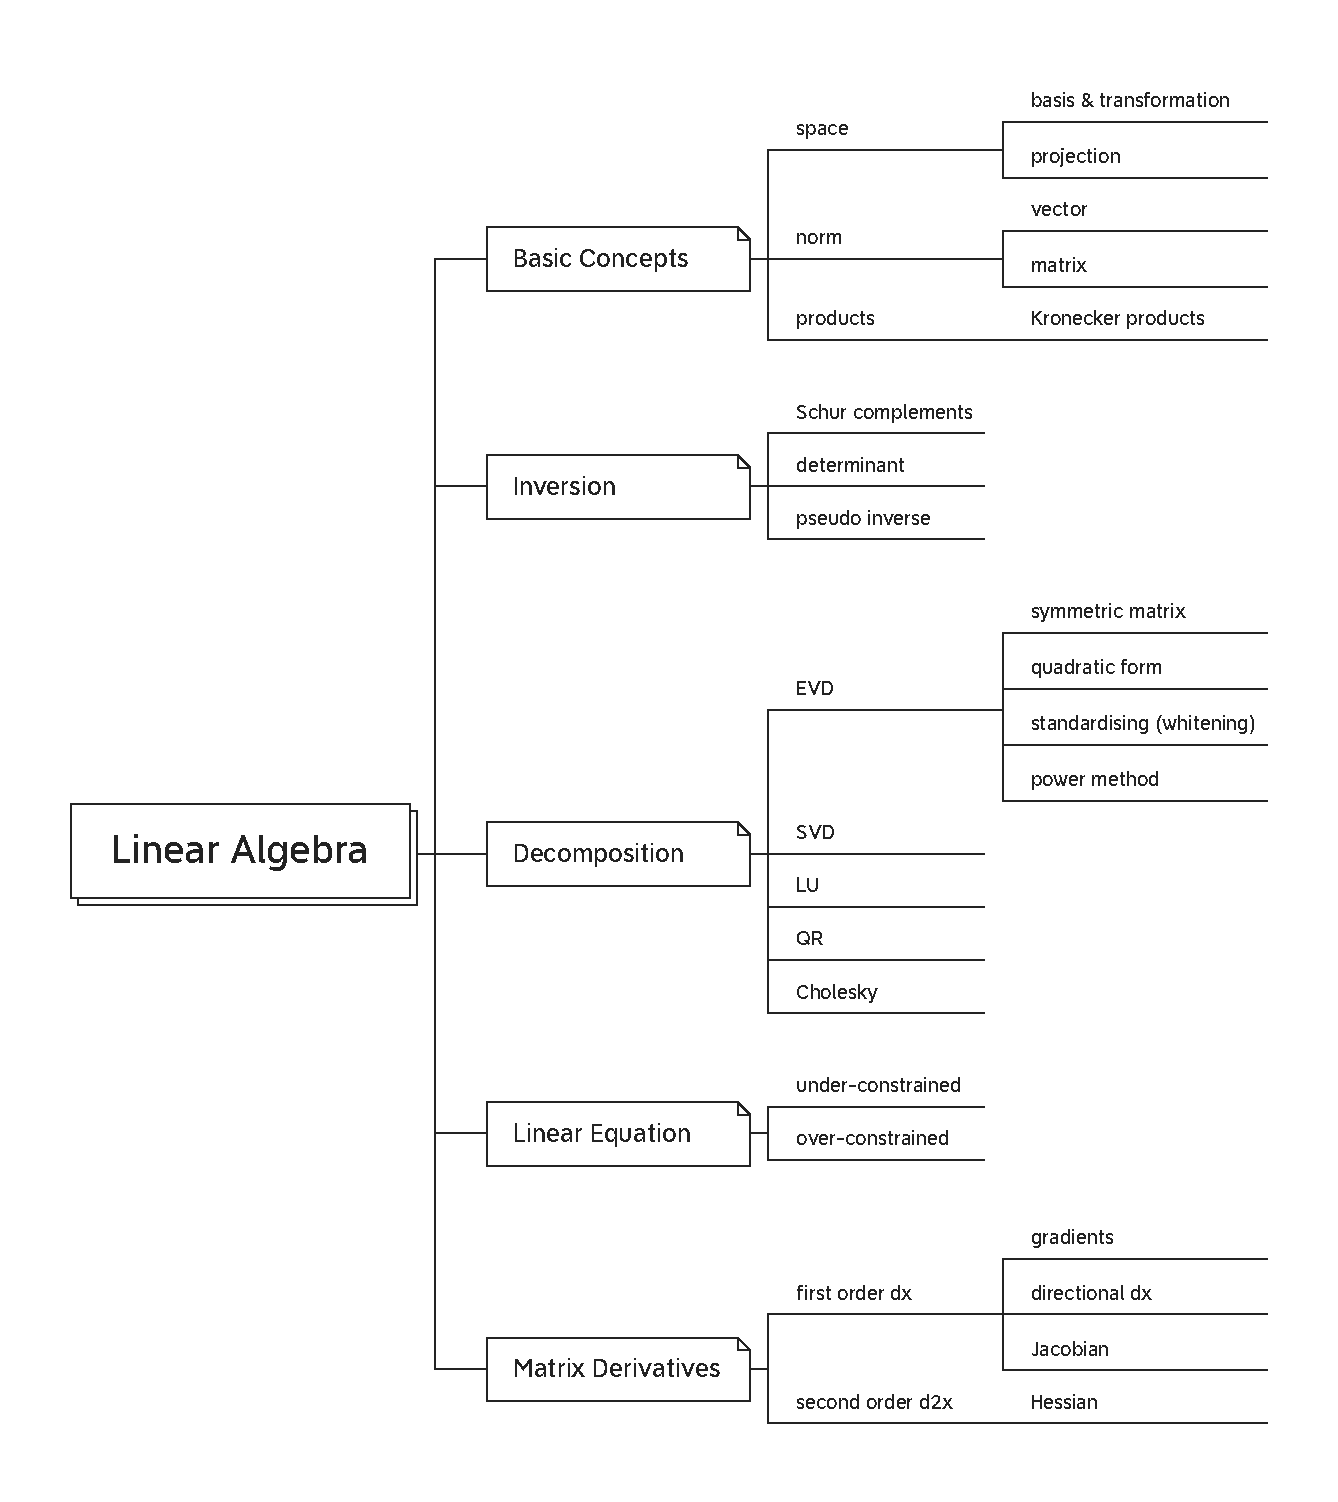
\includegraphics[width=.75\textwidth]{figs/linalgoutline.pdf}
%     \caption{outline of Chapter 7}
%     \label{fig:linalgoutline}
% \end{figure}

\begin{figure}[htpb]
    \centering
    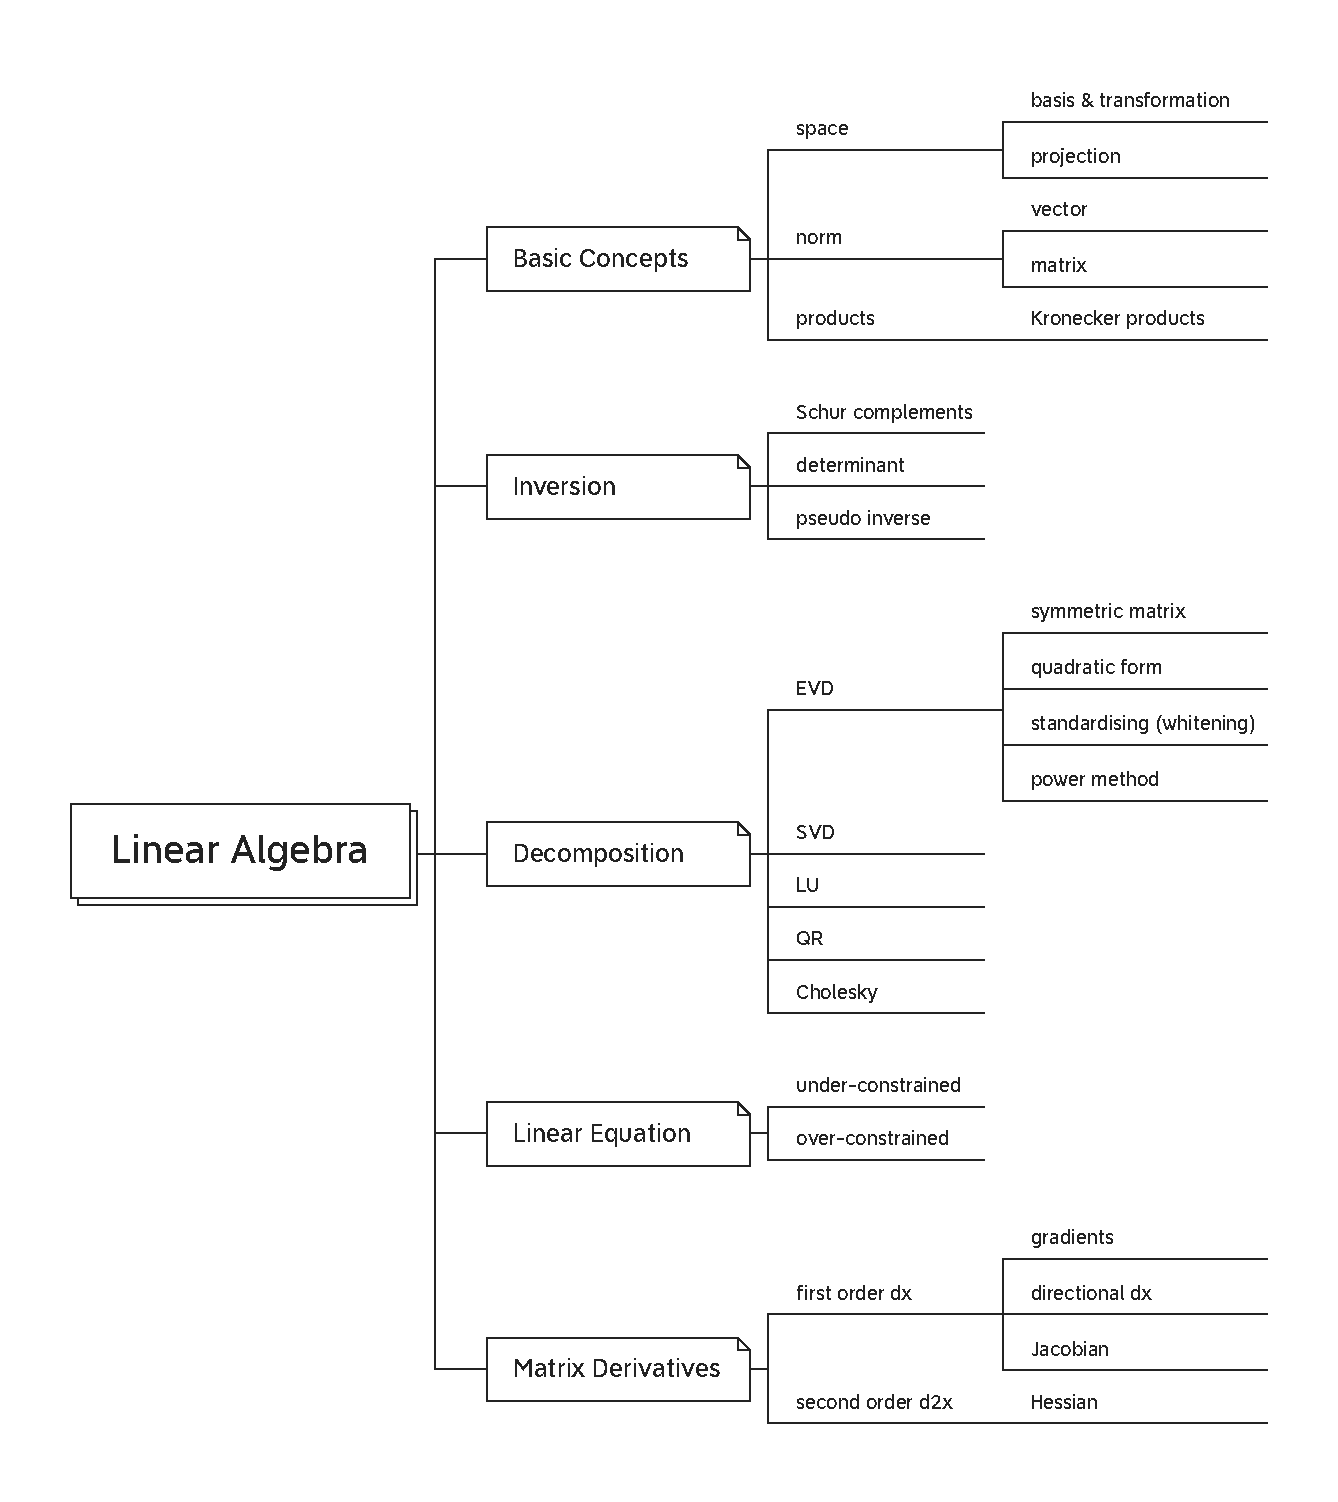
\includegraphics[width=.75\textwidth]{figs/linalgoutline.pdf}
    \caption{outline of Chapter 7}
    \label{fig:linalgoutline}
\end{figure}

Left-product operates rows and right-product operates columns.

\begin{table}[htpb]
    \centering
    \begin{tabular}{rp{24em}}
        \toprule
        Terminology & Definition \\
        \midrule
        
        \textbf{span} of vectors & $\text{span}(\{\bm{x}_1,\cdots,\bm{x}_n\})\triangleq\left\{\bm{v}:\bm{v}=\sum_{i=1}^n\alpha_i\bm{x}_i,\alpha_i\in\mathbb{R}\right\}$\\
    
        \textbf{range} of a matrix &
        $\text{range}(\mathbf{A})\triangleq\{\bm{v}=\mathbf{A}\bm{x}\}$, span of the column vectors, also named column space, a new space \\
    
        \textbf{nullspace} of a matrix & $\text{nullspace}(\mathbf{A})\triangleq{\{\bm{x}:\mathbf{A}\bm{x}=\bm{0}\}}$, subspace of the original space\\
        
        \textbf{max-norm} and \textbf{0-norm} &
        $\|\bm{x}\|_\infty=\max|x_i|$ and $\|\bm{x}\|_0=\sum_{i=1}^n\mathbb{I}(x_i\neq 0)$\\
        
        \textbf{element-wise square}                    & $\mathbf{A}^{\odot 2}$ \\
        \textbf{root of a matrix}                       & $\mathbf{M}\triangleq\sqrt{\mathbf{A}}$ if $\mathbf{M}^2=\mathbf{A}$ \\
        \textbf{summing slices of matrix}               & across row $\mathbf{1}_N^\mathsf{T}\mathbf{X}$, or across column $\mathbf{X1}_D$ \\
        \textbf{scaling a matrix}                       & scaling each row, $\mathrm{diag}(\bm{s})\mathbf{X}$, or each column, $\mathbf{X}\mathrm{diag}({\bm{s}})$. \\
        \textbf{shifting a matrix}                      & $\mathbf{X}-\mathbf{1}_N\bm{t}^\mathsf{T}$ \\
        
        \textbf{empirical mean}                         & $(\hat{\bm{\mu}}^\mathsf{T}=)\Bar{\bm{x}}^\mathsf{T}=\frac{1}{N}\mathbf{1}_N^\mathsf{T}\mathbf{X}$ \\
        \textbf{centering matrix}                       & $\mathbf{C}_N\triangleq\mathbf{I}_N-\frac{1}{N}\mathbf{J}_N$ idempotent\\
        \textbf{centered matrix}                        & $\Tilde{\mathbf{X}}=\mathbf{C}_N\mathbf{X}$ \\
        \textbf{scatter matrix}                         & 
        $(\hat{\mathbf{\Sigma}}=)\mathbf{S}_{\Bar{\bm{x}}}\triangleq\Tilde{\mathbf{X}}^\mathsf{T}\Tilde{\mathbf{X}}=\mathbf{X}^\mathsf{T}\mathbf{C}_N\mathbf{X}$ \\
        
        \textbf{distance matrix}                        & 
        $D_{ij}=(\bm{x}_i-\bm{y}_j)^\mathsf{T}(\bm{x}_i-\bm{y}_j)=\|\bm{x}_i\|^2-2\bm{x}_i^\mathsf{T}\bm{y}_j+\|\bm{y}_j\|^2$ \\
        \textbf{Kronecker products}                     & $\mathbf{A}_{m\times n}\otimes\mathbf{B}_{p\times q}=[a_{ij}\mathbf{B}]_{mp\times nq}$ {\color{red} what are its applications?} \\
        \textbf{Einstein summation}                     & for simplifying the notation, no new product rule, e.g. $E_{nd}={\color{gray}\sum_k\sum_t}S_{ntk}W_{kd}$,
        implemented in \texttt{opt\_einsum}, \texttt{numpy}, \texttt{torch}, \texttt{tensorflow}, and \texttt{jax}. \\
        \textbf{Schur complements}                      & If $\mathbf{M}=\left[\begin{array}{cc}
            \mathbf{E} & \mathbf{F} \\
            \mathbf{G} & \mathbf{H}
        \end{array}\right]$, then $\mathbf{M}/\mathbf{H}\triangleq\mathbf{E}-\mathbf{FH}^{-1}\mathbf{G}$ and $\mathbf{M}/\mathbf{E}\triangleq\mathbf{H}-\mathbf{GE}^{-1}\mathbf{F}$\\
        \textbf{M-P inverse}                            & $\mathbf{A}^\dag$ such that $\mathbf{AA}^\dag$ and $\mathbf{A}^\dag\mathbf{A}$ are symmetric,
        $\mathbf{AA}^\dag\mathbf{A}=\mathbf{A}$, and $\mathbf{A}^\dag\mathbf{AA}^\dag=\mathbf{A}^\dag$. 
        \uline{We can compute $\mathbf{A}^\dag=\mathbf{VS}^{-1}\mathbf{U}^\mathsf{T}$} \\
        \textbf{rank-nullity theorem}                   & $\text{rank} + \text{nullity} = n$, where nullity is the dim of nullspace, which can be proofed by SVD.\\
        \textbf{LU decomposition}                       & $\mathbf{PA}=\mathbf{LU}$, where $\mathbf{P}$ is a permutation matrix that permutes row $j$ to row $i$ if $P_{ij}=1$ (partial pivoting).\\
        \textbf{directional derivative}                 & {\footnotesize For $f:\mathbb{R}^n\to\mathbb{R}$, 
        $D_{\bm{v}}f(\bm{x})=\lim_{h\to 0}\frac{f(\bm{x}+h\bm{v})-f(\bm{x})}{h}=\nabla f(x)\cdot \bm{v}$} \\
        \textbf{Jabobian}                               & {\footnotesize For $\bm{f}:\mathbb{R}^n\to\mathbb{R}^m$,
        $\mathbf{J}_{\bm{f}(\bm{x})}
        = \frac{\partial{\bm{f}}}{\partial{\bm{x}^\mathsf{T}}}
        \triangleq\left[\frac{\partial{f_i}}{\partial{x_j}}\right]
        = \left[\nabla f_i(\bm{x})^\mathsf{T}\right]\in\mathbb{R}^{m\times n}$} \\
        \textbf{Hessian}                                & {\footnotesize For $f:\mathbb{R}^n\to\mathbb{R}$,
        $\mathbf{H}_f=\frac{\partial^2 f}{\partial\bm{x}^2}=\nabla^2 f=\left[\frac{\partial^2 f}{\partial x_ix_j}\right]\in\mathbb{R}^{n\times n}$}\\
        \textbf{Lipschitz constant}                     & $\{L:|f(x_1)-f(x_2)|\leq{L}|x_1-x_2|,\forall{x_1,x_2}\}$, qualifying the degree of smoothness of a function $f$. \\
        \textbf{perplexity}                             & $\text{perplexity}(p)\triangleq 2^{\mathbb{H}(p)}$, a measure of predictability, and $\text{perplexity}(p_\mathcal{D},p)\triangleq 2^{\mathbb{H}_\text{ce}(p_\mathcal{D},p)}$, a measure how well $p$ predicts $\mathcal{D}$ \\
        \bottomrule
    \end{tabular}
    \caption{Brief concepts}
    \label{tab:linalg}
\end{table}



% \begin{itemize}
%     \item 
% \end{itemize}

\textbf{basis}:
$\mathcal{B}$, a set of vectors (independent of course and \textbf{coordinate vectors} by default) 
that can span the \textit{whole space}.
The vectors we used in theory or application can be interpreted as the real coordinates in a standard  



\textbf{projection}: find a vector \textit{nearest} to the given vector in the given (spanned) space
\begin{gather}
    \text{Proj}(\bm{y};\{\bm{x}_1,\cdots,\bm{x}_n\})
    =\argmin_{\bm{v}\in\text{span}(\{\bm{x}_1,\cdots,\bm{x}_n\})}\|\bm{y}-\bm{v}\|_2\label{eq:proj}
\end{gather}\unsure{
2-norm in the definition is the key linking OLS, with squared loss, to projection.}
If $\mathbf{A}$ full rank in columns:
\begin{gather}
    \mathrm{Eq(\ref{eq:proj})}=\text{Proj}(\bm{y};\mathbf{A})
    =\mathbf{A}(\mathbf{A}^\mathsf{T}\mathbf{A})^{-1}\mathbf{A}^\mathsf{T}\bm{y}
\end{gather}
which can means to find a vector $\bm{v}$ in the column space of $\mathbf{A}$ 
such that $\bm{v}$ is as close as possible to $\bm{y}$,
minimizing the \textit{squared} error of the feasible representation space.

\textbf{Vector norm}:
$\|\bm{x}\|:\mathbb{R}^n\to\mathbb{R}$, \textit{a} measure of \textit{length} of the vector.\unsure{
any function satisfying the properties of distance can serve as norm.
Recall the definition of measure in set theory. 
Norm is a special \textbf{measure} of any rectangular interval in topological space.
}
The most used norm is \textbf{p-norm}
\begin{gather}
    \|\bm{x}\|_p=\left[\sum_{i=1}^D |x_i|^p\right]^\frac{1}{p},~p\geq{1}
\end{gather}
which is Euclidean distance when $p=2$ or maximal element when $p=\infty$. 
The case of $p=0$ is defined specially as the number of non-zero elements in $\bm{x}$

\textbf{Matrix norm} (with definitions in diversity):
\begin{enumerate}[{(1)}]
    \item \textbf{induced norm}: 
    the maximum response of a linear function $\mathbb{A}\bm{x}$ by unite-norm input under p-norm, the measure of length for input and response \unsure{
    recall that the \textbf{norm of a vector} is a measure of the vector's length or magnitude
    and the singular value of a matrix is magnitude rate along axes in a rotated space}
    \begin{gather}
        \|\mathbf{A}\|_p
        = \max_{\bm{x}\neq\bm{0}}\frac{\|\mathbf{A}\bm{x}\|_p}{\|\bm{x}\|_p}
        = \max_{\|\bm{x}\|_p=1}\|\mathbf{A}\bm{x}\|_p\\
        \|\mathbf{A}\|_2
        = \sqrt{\lambda_{\text{max}}(\mathbf{A}^\mathsf{T}\mathbf{A}))}
        = \sqrt{\|\bm{\lambda}(\mathbf{A}^\mathsf{T}\mathbf{A})\|_\infty}
        = \|\bm{\sigma}(\mathbf{A})\|_\infty
    \end{gather}
    
    \item \textbf{nuclear norm} or \textbf{trace norm}: 
    \begin{gather}
        \|\mathbf{A}\|_*
        = \mathrm{tr}(\sqrt{\mathbf{A}^\mathsf{T}\mathbf{A}})
        = \sum_i\sigma_i
        = \sum_i|\sigma_i|
        = \|\bm{\sigma}\|_1
    \end{gather}
    To regularize model with this norm, low rank parameter matrix will be reached.
    
    \item \textbf{Schatten p-norm}: generalize the nuclear norm, 
    equal to 1-norm, to p-norm on the singular vector of $\mathbf{A}$
    \begin{gather}
        \|\mathbf{A}\|_p=\|\bm{\sigma}(\mathbf{A})\|_p
    \end{gather}
    Induced 2-norm and Schatten $\infty$-norm are the same.
    
    \item \textbf{Frobenius norm}: treat the matrix as a vector and apply 2-norm
    \begin{gather}
        \|\mathbf{A}\|_F
        = \sqrt{\sum_{i=1}^m\sum_{j=1}^n{a_{ij}^2}}
        = \|\mathrm{vec}(\mathbf{A})\|_2
        = \sqrt{\mathrm{tr}(\mathbf{A}^\mathsf{T}\mathbf{A})}
    \end{gather}
    For a random vector $\bm{v}\sim\mathcal{N}(\mathbf{0},\mathbf{I})$,
    \begin{gather}
        \|\mathbf{A}\|_F^2
        = \mathrm{tr}(\mathbf{A}^\mathsf{T}\mathbf{A})
        = \mathbb{E}(\bm{v}^\mathsf{T}\mathbf{A}^\mathsf{T}\mathbf{A}\bm{v})
        = \mathbb{E}\|\mathbf{A}\bm{v}\|_2^2
        \approx \frac{1}{n}\sum_{i=1}^N\|\mathbf{Av}_i\|_2^2 \label{eq:forbnormapprox}
    \end{gather}
    when $\mathbf{A}$ is expensive but $\mathbf{A}\bm{v}$ cheap to evaluate, 
    Equation (\ref{eq:forbnormapprox}) can be used to approximate Frobenius norm.
\end{enumerate}

Properties of \textbf{trace}: $\mathrm{tr}(\mathbf{A})\triangleq\sum_{i=1}^n A_{ii}$:
\begin{enumerate}[{(1)}]
    \item trace and eigenvalues: $\mathrm{tr}(\mathbf{A})=\sum_{i=1}^n\lambda_i$
    
    \item cyclic permutation property: $\mathrm{tr}(\mathbf{ABC})=\mathrm{tr}(\mathbf{BCA})=\mathrm{tr}(\mathbf{CAB})$
    
    \item trace trick: $\bm{x}^\mathsf{T}\mathbf{A}\bm{x}=\mathrm{tr}(\bm{x}^\mathsf{T}\bm{x}\mathbf{A})$\unsure{
    The result is scaler, memory used in LHS: $n+n^2+n\rightarrow n+n\rightarrow 1$, 
    and in RHS: $n+n+n^2\rightarrow n^2+n^2\rightarrow n^2\rightarrow 1$.
    }
    and \textbf{Hutchinson trace estimator} (similar to Equation (\ref{eq:forbnormapprox})):
    For any random vector $\bm{v}$ such that $\mathbb{E}(\bm{vv}^\mathsf{T})=\mathbf{I}$
    \begin{gather}
        \mathrm{tr}(\mathbf{A})
        = \mathrm{tr}(\mathbf{A}\mathbb{E}(\bm{vv}^\mathsf{T}))
        = \mathbb{E}[\mathrm{tr}(\bm{v}^\mathsf{T}\mathbf{A}\bm{v})]
    \end{gather}
\end{enumerate}

Properties of \textbf{determinant}: 
$\mathrm{det}(\mathbf{A})$ or $|\mathbf{A}|$ is a measure of how much it changes a unit volume when viewed as a linear transformation.\unsure{
Recall the transformation of multiple r.v.s.
}
\begin{enumerate}[{(1)}]
    \item determinant and eigenvalues: $|\mathbf{A}|=\prod_{i=1}^n\lambda_i$. 
    \textit{proof}: 
    $\exists$ unit orthogonal matrix $\mathbf{V}$ ($\mathbf{V}^\mathsf{T}=\mathbf{V}^{-1}$) 
    for any $\mathbf{A}$ 
    such that $\mathbf{A}=\mathbf{V\Lambda V}^\mathsf{T}$,
    so
    \begin{gather}
        |\mathbf{A}|=|\mathbf{VV}^\mathsf{T}\mathbf{\Lambda}|=|\mathbf{1}||\mathbf{\Lambda}|=\prod_{i=1}^n\lambda_i
    \end{gather}
    
    \item positive definite matrix can be written as $\mathbf{A}=\mathbf{LL}^\mathsf{T}$, 
    where $\mathbf{L}$ is the \textbf{lower triangular Cholesky decomposition}:
    \begin{gather}
        |\mathbf{A}|=|\mathbf{L}|^2 \Rightarrow\\
        \log{|\mathbf{A}|}=2\log\prod_{i=1}^n L_{ii}=2~\mathrm{tr}(\log\mathrm{diag}(\mathbf{L}))
    \end{gather}
\end{enumerate}

\textbf{Rank of a matrix}: there are various definitions that can be used according to the application contexts:
\begin{enumerate}[{(1)}]
    \item \uline{$\mathrm{columnrank}(\mathbf{A})=\mathrm{rowrank}(\mathbf{A})=\mathrm{rank}(\mathbf{A})$},
    where column/row rank of a matrix is the dimension of the space spanned by its columns/rows
    
    \item \textbf{factorization rank}:
    \begin{gather}
        \mathbf{A}=\mathbf{CR},~\mathbf{C}\in\mathbb{R}^{m\times{k}}\Rightarrow
        \mathrm{rank}(\mathbf{A})=\inf{k}
    \end{gather}
    
    \item \textbf{SVD decomposition rank}:
    \begin{gather}
        \mathbf{A}=\mathbf{U\Sigma V}\Rightarrow
        \mathrm{rank}(\mathbf{A})=\#\{\bm{\sigma}\neq 0\}
    \end{gather}
\end{enumerate}

Properties of rank: For $\mathbf{A}$ with order $m\times n$\unsure{
this properties are useful in STAT5030, and it will keep updating later.}
\begin{enumerate}[{(1)}]
    \item $\mathrm{rank}(\mathbf{A})\leq\min\{m,n\}$, 
    $\mathbf{A}$ called \textbf{full rank} if the equality holds else \textbf{rank deficient}.
    \item $\mathbf{A}$ square: $\mathbf{A}$ invertible $\iff$ $\mathbf{A}$ nonsingular $iff$ $\mathbf{A}$ full rank.
    \item $\mathrm{rank}(\mathbf{A})=\mathrm{rank}(\mathbf{AA}^\mathsf{T})=\mathrm{rank}(\mathbf{A}^\mathsf{T}\mathbf{A})$.
    \item $\mathrm{rank}(\mathbf{AB})\leq\min\{\mathrm{rank}(\mathbf{A}),\mathrm{rank}(\mathbf{B})\}$, the equality holds if $\mathrm{rank}(\mathbf{B})=n$.
    \item $\mathrm{rank}(\mathbf{A}+\mathbf{B})\leq\mathrm{rank}(\mathbf{A})+\mathrm{rank}(\mathbf{B})$.
    \item $\exists \mathbf{P}$ with order $m\times{m}$ and $\mathbf{Q}$ with order $n\times n$, both invertible such that 
    \begin{gather}
        \mathbf{PAQ}=\left[\begin{array}{cc}
            \mathbf{I}_r & \mathbf{0} \\
            \mathbf{0} & \mathbf{0}
        \end{array}\right]
    \end{gather}
\end{enumerate}

\textbf{Condition number} of a matrix $\mathbf{A}$
\begin{gather}
    \kappa(\mathbf{A})
    \triangleq \|\mathbf{A}\|\|\mathbf{A}^{-1}\|
    = \frac{\sigma_{\text{max}}}{\sigma_{\text{min}}}
    = \sqrt{\frac{\lambda_{\text{max}}}{\lambda_{\text{min}}}}
\end{gather}
measures the numerical stability of any computations involving $\mathbf{A}$ ($\Delta\bm{x}=\mathbf{A}^{-1}\Delta\bm{b}$) 
or the nearness to singularity.
The condition number depends on the norm used (induced $\ell_2$-norm by default).

\textbf{Orthogonal matrix} $\mathbf{U}\in\mathbb{R}^{n\times n}$ such that 
for any $\bm{x}$ and $\bm{y}$ are both column (or row) vectors of $\mathbf{U}$
\begin{gather}
    \underbrace{\bm{x}^\mathsf{T}\bm{y}=0}_{\text{orthogonal}}
    ~\text{and}~
    \underbrace{\|\bm{x}\|_2=1}_{\text{normalized}},
\end{gather}
which satisfies $\mathbf{U}^\mathsf{T}=\mathbf{U}^{-1}$.
Transformations by $\mathbf{U}$ are rigid (no deformation locally or globally), 
i.e. rotations or reflections if $|\mathbf{U}|=1$ or $-1$.

\textbf{Gram matrix} $\mathbf{K}$ depicts the features' linear similarity of samples, used as kernel in linear SVM.\unsure{
Note the difference with distance matrix $\mathbf{D}=\hat{\bm{x}}\mathbf{1}_N^\mathsf{T}-2\mathbf{K}+\mathbf{1}_N\hat{\bm{x}}^\mathsf{T}$,
which measure the discrepancy between samples (each row in $\mathbf{X}$), where $\hat{\bm{x}}=\mathrm{diag}(\mathbf{XX}^\mathsf{T})$.
}
\begin{gather}
    \mathbf{K}\triangleq\mathbf{XX}^\mathsf{T}\\
    \Tilde{\mathbf{K}}=\Tilde{\mathbf{X}}\Tilde{\mathbf{X}}^\mathsf{T}=\mathbf{C}_N\mathbf{KC}_N
\end{gather}

\textbf{Orthogonal matrix's geometric interpret in eigenvalue decomposition}:
Recall the EVD for any square matrix $\mathbf{A}$: $\mathbf{AU}=\mathbf{U\Lambda}$,
where columns of $\mathbf{U}$ are corresponding eigenvectors.
If $\mathbf{U}$ is invertible, then $\mathbf{A}=\mathbf{U\Lambda U}^{-1}$ and is called \textbf{diagonalizable}.
If $\mathbf{A}$ is real and symmetric, then $\mathbf{A}=\mathbf{U\Lambda U}^\mathsf{T}$, 
implying $\mathbf{U}$ is an orthogonal matrix.

Any real symmetric matrix $\mathbf{A}$ can be interpreted as multiplying by 
a rotation matrix $\mathbf{U}^\mathsf{T}$, a scaling matrix $\mathbf{\Lambda}$, followed by an inverse rotation $\mathbf{U}$,
and its inverse, easily as $\mathbf{A}^{-1}=\mathbf{U\Lambda}^{-1}\mathbf{U}^\mathsf{T}$, 
corresponds to rotating, unscaling, and then rotating back.

\begin{example}
    \item \textbf{Geometry of quadratic form}: The eigenvectors determine
    the \textit{orientation} of the ellipse, and the eigenvalues determine how \textit{elongated} it is.
    \begin{gather}
        f(\bm{x})=\bm{x}^\mathsf{T}\mathbf{A}\bm{x}=\bm{x}^\mathsf{T}\mathbf{U\Lambda U}^\mathsf{T}\bm{x}
        =\bm{y}^\mathsf{T}\mathbf{\Lambda}\bm{y}=\sum_{d=1}^D \lambda_d y_d^2.
    \end{gather}
    The eigenvalues can be used to check positive definiteness quickly. 
\end{example}

\begin{example}
    \textbf{Standardizing and whitening data}: 
    preprocess the data so that each column has zero mean and unit variance, 
    and remove correlation between the columns (by rotating the coordinate).
    Assume $\mathbf{X}\in\mathbb{R}^{N\times D}$ is standardized,
    then 
    \begin{gather}
        \mathbf{EDE}^\mathsf{T}=\hat{\mathbf{\Sigma}}=\frac{1}{N}\mathbf{X}^\mathsf{T}\mathbf{X} \\
        \bm{y}=\mathbf{W}\bm{x}
    \end{gather}
    where $\mathbf{W}=\mathbf{W}_\text{pca}=\mathbf{D}^{-\frac{1}{2}}\mathbf{E}^\mathsf{T}$ (\uline{rotate and scale}) if PCA whiten, or
    $\mathbf{W}=\mathbf{W}_\text{zca}=\mathbf{E}\mathbf{D}^{-\frac{1}{2}}\mathbf{E}^\mathsf{T}=\mathbf{\Sigma}^{-\frac{1}{2}}$ (\uline{rotate, scale, and rotate back}) if Mahalanobis whiten,
    which is similar to the Mahalanobis distance.
\end{example}

\begin{example}
    \textbf{Power method}: a \textit{iterative} method for computing the \textit{largest eigenvalue's eigenvector} for a real, \textit{symmetric} matrix,
    useful for very \textit{large but sparse} matrix.
    \begin{align}
        \bm{v}_{t}\propto&\mathbf{A}\bm{v}_{t-1}\\
        \Rightarrow
        \bm{v}_{t}\propto&\mathbf{A}^t\bm{v}_0\\
        =& a_1\lambda_1^t\bm{u}_1+\cdots+a_n\lambda_n^t\bm{u}_n\\
        =& \lambda_1^t(a_1\bm{u}_1+\cdots+a_m(\frac{\lambda_n}{\lambda_1})^t\bm{u}_n)\\
        \to& \lambda_1^ta_1\bm{u}_1~\text{as}~t\to\infty\\
        \lambda_i=&\frac{\bm{u}_i^\mathsf{T}\mathbf{A}\bm{u}_i}{\bm{u}_i^\mathsf{T}\bm{u}_i}\triangleq R(\mathbf{A},\bm{u}_i)~(\textbf{Rayleigh quotient})
    \end{align}
\end{example}

\textbf{Singular value decomposition} (SVD):
Any real rectangular $m\times n$ matrix $\mathbf{A}$ can be decomposed as
\begin{gather}
    \mathbf{A}=\mathbf{USV}^\mathsf{T}
\end{gather}
where $\mathbf{U}\in\mathbb{R}^{m\times m}$ and $\mathbf{V}\in\mathbb{R}^{n\times n}$ are both orthogonal matrix,
and the bigger one is not unique and has irrelevant columns that can be set as all 0, then called economy sized or thin SVD.
\begin{gather}
    \mathbf{A}^\mathsf{T}\mathbf{A}=\mathbf{V}(\mathbf{S}^\mathsf{T}\mathbf{S})\mathbf{V}^\mathsf{T}\\
    \mathbf{AA}^\mathsf{T}=\mathbf{U}(\mathbf{SS}^\mathsf{T})\mathbf{U}^\mathsf{T}
\end{gather}
It is worth noting that the singular values of SVD are sorted from big to small in $\mathbf{S}$.
\textbf{Truncated SVD} only keeps the first $K$ singular values in $\mathbf{S}$ 
and first $K$ columns of $\mathbf{U}$ and $\mathbf{V}$
\begin{gather}
    \hat{\mathbf{A}}_K=\mathbf{U}_K\mathbf{S}_K\mathbf{V}_K^\mathsf{T},
\end{gather}
which will incur some error if $K<\mathrm{rank}(\mathbf{A})$, and the error is given by
\begin{gather}
    \text{error}=\|\mathbf{A}-\hat{\mathbf{A}}_K\|_F=\sum_{k=K+1}^{\mathrm{rank}(\mathbf{A})}\sigma_k
\end{gather}\unsure{
The error is evaluated by Frobenius norm.
}

\textbf{QR decomposition}: representing a set of linearly independent basis vectors (so $m \geq n$) $\bm{q}_i$ and their coefficients $r_{ij}$ 
\begin{gather}
    \mathbf{A}=\hat{\mathbf{Q}}\hat{\mathbf{R}}
\end{gather}
where $\hat{\mathbf{Q}}\in\mathbb{R}^{m\times n}$ with orthonormal columns and $\hat{\mathbf{R}}\in\mathbb{R}^{n\times n}$ is upper triangular,
and such case ia called \textbf{economy size QR}.
For \textbf{full QR}, we complement the complete orthonormal columns $\Tilde{\mathbf{Q}}\in\mathbb{R}^{m\times(m-n)}$ to $\hat{\mathbf{Q}}$ and additional ``0'' entries to $\hat{\mathbf{R}}$
\begin{gather}
    \mathbf{A}
    = \mathbf{QR}
    = \left[\begin{array}{cc}
        \hat{\mathbf{Q}} & \Tilde{\mathbf{Q}}
    \end{array}\right]
    \left[\begin{array}{cc}
        \hat{\mathbf{R}} & \mathbf{0} \\
        \mathbf{0} & \mathbf{0}
    \end{array}\right]\\
    \mathbf{Q},\mathbf{R}\in\mathbb{R}^{m\times m}
\end{gather}


\textbf{Cholesky decomposition}: for any symmetric $\mathbf{A}$
\begin{gather}
    \mathbf{A}=\mathbf{R}^\mathsf{T}\mathbf{R}=\mathbf{LL}^\mathsf{T},
\end{gather}
which is used to generate r.v.s with designed covariance.

\begin{example}
    \textbf{Sampling from an MVN with specified covariance matrix} $\mathbf{\Sigma}$\\
    \begin{gather}
        \bm{x}\sim\mathcal{N}(\mathbf{0},\mathbf{I})\\
        \bm{y}=\mathbf{L}\bm{x}+\bm{\mu}\sim\mathcal{N}(\bm{\mu},\mathbf{\Sigma})
    \end{gather}
\end{example}

\textbf{Linear equation system}: 
we have $\mathbf{A}\in\mathbb{R}^{m\times n}$ samples of observed variables, 
and $\bm{b}\in\mathbb{R}^{m\times m}$ samples' measured responds, and 
$\bm{x}\in\mathbb{R}^{n\times 1}$ coefficients of variables to be estimated
\begin{gather}
    \mathbf{A}\bm{x}=\bm{b}
\end{gather}
which is \textbf{over-determined} and there are multiple solutions if $m<n$:
\begin{gather}
    \{\bm{x}: \mathbf{A}\bm{x}=\bm{b}\}
    = \{\underbrace{\mathbf{A}^\mathsf{T}(\mathbf{AA}^\mathsf{T})^{-1}}_{\text{right inverse}}\bm{b}+\bm{z}:\bm{z}\in\mathrm{nullspace}(\mathbf{A})\}
\end{gather}
or \textbf{under-determined} and there is not exact solution but \textbf{ordinary least squares} (OLS) solution with minimal error if $m>n$:
\begin{gather}
    \hat{\bm{x}} = \underbrace{(\mathbf{A}^\mathsf{T}\mathbf{A})^{-1}\mathbf{A}^\mathsf{T}}_{\text{left inverse}}\bm{b}
\end{gather}

\textbf{Matrix and vector's calculus}:
\begin{enumerate}[{(1)}]
    \item $f:\mathbb{R}^n\to\mathbb{R}$:
    \begin{enumerate}
        \item $\nabla(\bm{a}^\mathsf{T}\bm{x})=\bm{a}$
        \item $\nabla(\bm{b}^\mathsf{T}\mathbf{A}\bm{x})=\mathbf{A}^\mathsf{T}\bm{b}$
        \item $\nabla(\bm{x}^T\mathbf{A}\bm{x})=(\mathbf{A}+\mathbf{A}^\mathsf{T})\bm{x}$
    \end{enumerate}
    \item $f:\mathbb{R}^{m\times n}\to\mathbb{R}$: $\frac{\partial{f}}{\partial\mathbf{X}}=\left[\frac{\partial{f}}{\partial{x_{ij}}}\right]\in\mathbb{R}^{m\times n}$
    \begin{enumerate}
        \item $\frac{\partial}{\partial{\mathbf{X}}}(\bm{a}^\mathsf{T}\mathbf{X}\bm{b})=\bm{ab}^\mathsf{T}$
        \item $\frac{\partial}{\partial{\mathbf{X}}}(\bm{a}^\mathsf{T}\mathbf{X}^\mathsf{T}\bm{b})=\bm{ba}^\mathsf{T}$
        \item $\frac{\partial}{\partial{\mathbf{X}}}\mathrm{tr}(\mathbf{AXB})=\mathbf{A}^\mathsf{T}\mathbf{B}^\mathsf{T}$
        \item $\frac{\partial}{\partial{\mathbf{X}}}\mathrm{tr}(\mathbf{X}^\mathsf{T}\mathbf{A})=\mathbf{A}$
        \item $\frac{\partial}{\partial{\mathbf{X}}}\mathrm{tr}(\mathbf{X}^{-1}\mathbf{A})=-\mathbf{X}^{-\mathsf{T}}\mathbf{A}^\mathsf{T}\mathbf{X}^{-\mathsf{T}}$
        \item $\frac{\partial}{\partial{\mathbf{X}}}\mathrm{tr}(\mathbf{X}^\mathsf{T}\mathbf{AX})=(\mathbf{A}+\mathbf{A}^\mathsf{T})\mathbf{X}$
        \item $\frac{\partial}{\partial{\mathbf{X}}}\mathrm{det}(\mathbf{AXB})=\mathrm{det}(\mathbf{AXB})\mathbb{X}^{-\mathsf{T}}$
        \item $\frac{\partial}{\partial{\mathbf{X}}}\log\mathrm{det}(\mathbf{X})=\mathbf{X}^{-\mathsf{T}}$
    \end{enumerate}
\end{enumerate}

\subsection{Optimization}

\textbf{Standard form of optimization}
\begin{gather}
    \bm{\theta}^*\in\argmin_{\bm{\theta}\in\mathcal{C}}\mathcal{L}(\bm{\theta})\\
    \mathcal{C}=\left\{
        \bm{\theta}: \bm{g}(\bm{\theta})\leq{\bm{0}},\bm{h}(\bm{\theta})=\bm{0}
    \right\}\in\mathbb{R}^D,
\end{gather}
where $\mathcal{L}$ is \textbf{optimization objective} and $\mathcal{C}$ is $\textbf{feasible set}$ 
in which $\bm{g}$ are inequality constrains and $\bm{h}$ are equality constrains.
Its the \textbf{generalized Lagrangian} is 
\begin{gather}
    L(\bm{\theta},\bm{\mu},\bm{\lambda})
    = \mathcal{L}(\bm{\theta})+\bm{\mu}^\mathsf{T}\bm{g}(\bm{\theta})+\bm{\lambda}^\mathsf{T}\bm{h}(\bm{\theta})\\
    \bm{\theta}^*= \min_{\bm{\theta}}\max_{\bm{\mu}\geq{\bm{0}},\bm{\lambda}}L(\bm{\theta},\bm{\mu},\bm{\lambda}).
\end{gather}
When both the objective and the constrain are convex, 
then a feasible solution $\bm{\theta}^*$ is global optimum \uline{if and only if} $\bm{\theta}^*$ satisfies the following 
\textbf{Karush-Kuhn-Tucker (KKT)} conditions:
{\small\begin{gather}
    \left\{\begin{array}{ll}
        \nabla_{\bm{\theta}}{L}=\nabla\mathcal{L}(\bm{\theta}^*)+\bm{\mu}^\mathsf{T}\nabla\bm{g}(\bm{\theta}^*)+\bm{\lambda}^\mathsf{T}\nabla\bm{h}(\bm{\theta}^*)=\bm{0} 
        & (\text{Lagrangian gradient wrt}~\bm{\theta})\\
        \bm{\mu}\geq\bm{0} 
        & \text{(dual feasibility)} \\
        \bm{\mu}\odot\bm{g}(\bm{\theta}^*)=\bm{0}
        & \text{(complementary slackness)} \\
    \end{array}\right.
\end{gather}}

\textbf{Subgradient}: generalize the gradient of the function (convex in optimization problem) with local discontinuities.
A\unsure{
At the discontinuous point, the subgradient may be not unique.
Any slop of the hyperplane that get through this discontinuous point and segment the space such that the convex function value is above
the hyperplane can serve as the subgradient at theis point, 
of course, if there exists such vector (subdifferentiable).
}
subgradient $\bm{g}\in\mathbb{R}^n$ at $\bm{x}_0$ of convex function $f:\mathbb{R}^n\to\mathbb{R}$ satisfies
\begin{gather}
    \bm{g}\in\{\bm{g}:f(\bm{x})\geq f(\bm{x}_0)+\bm{g}^\mathsf{T}(\bm{x}-\bm{x}_0)\}
\end{gather}

% \begin{figure}[htpb]
%     \centering
%     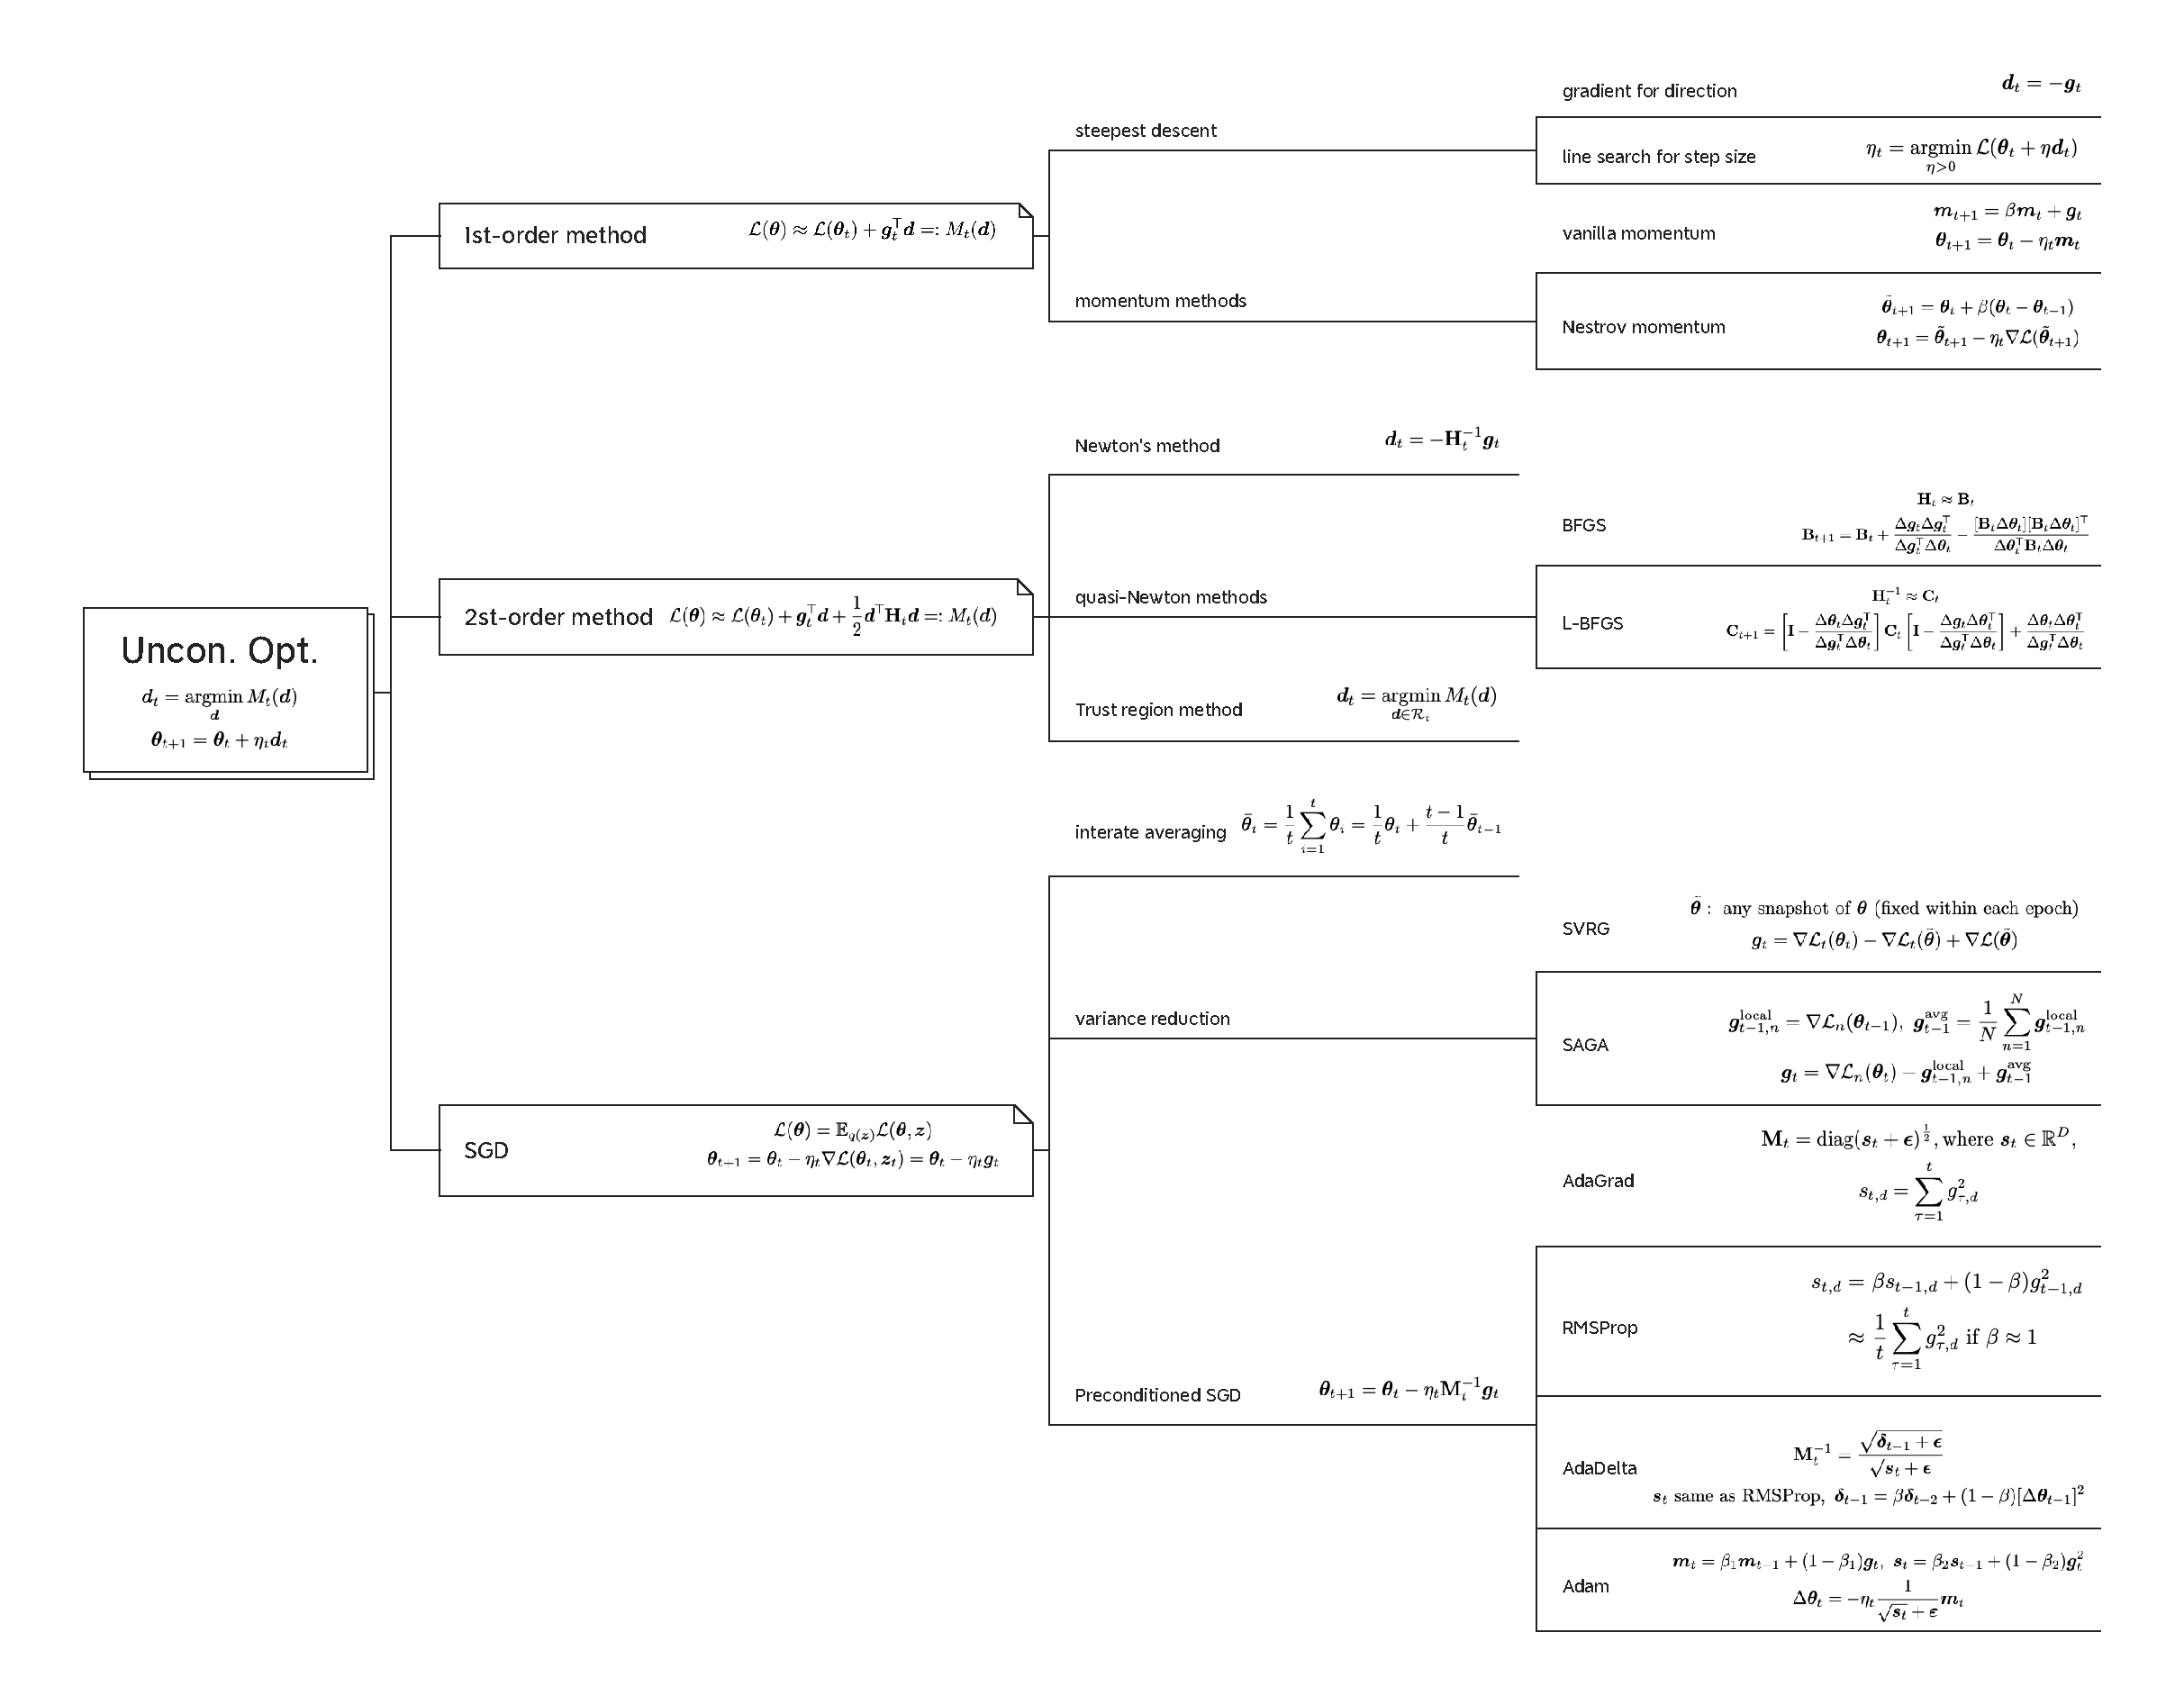
\includegraphics[width=\textwidth]{figs/unconopt.pdf}
%     \caption{Solutions for unconstrained optimization updating strategies}
%     {\footnotesize there are approximation methods for $M_t(\bm{d})$ and $\bm{d}_t$.
%     \textbf{BFGS}: Broyden, Fletcher, Goldfarb and Shanno;
%     \textbf{L-BFGS}: limited memory BFGS;
%     \textbf{SGD}: Stochastic Gradient Descent;
%     \textbf{SVRG}: Stochastic Variance Reduced Gradient;
%     \textbf{SAGA}: Stochastic Averaged Gradient Accelerated;
%     \textbf{AdaGrad}: ADAptive Gradient;
%     \textbf{RMSProp}: Root Mean Squared resilient PROPagation;
%     \textbf{Adam}: Adaptive moment estimation.
%     }
    
%     \label{fig:unconopt}
% \end{figure}

\begin{figure}[htpb]
    \centering
    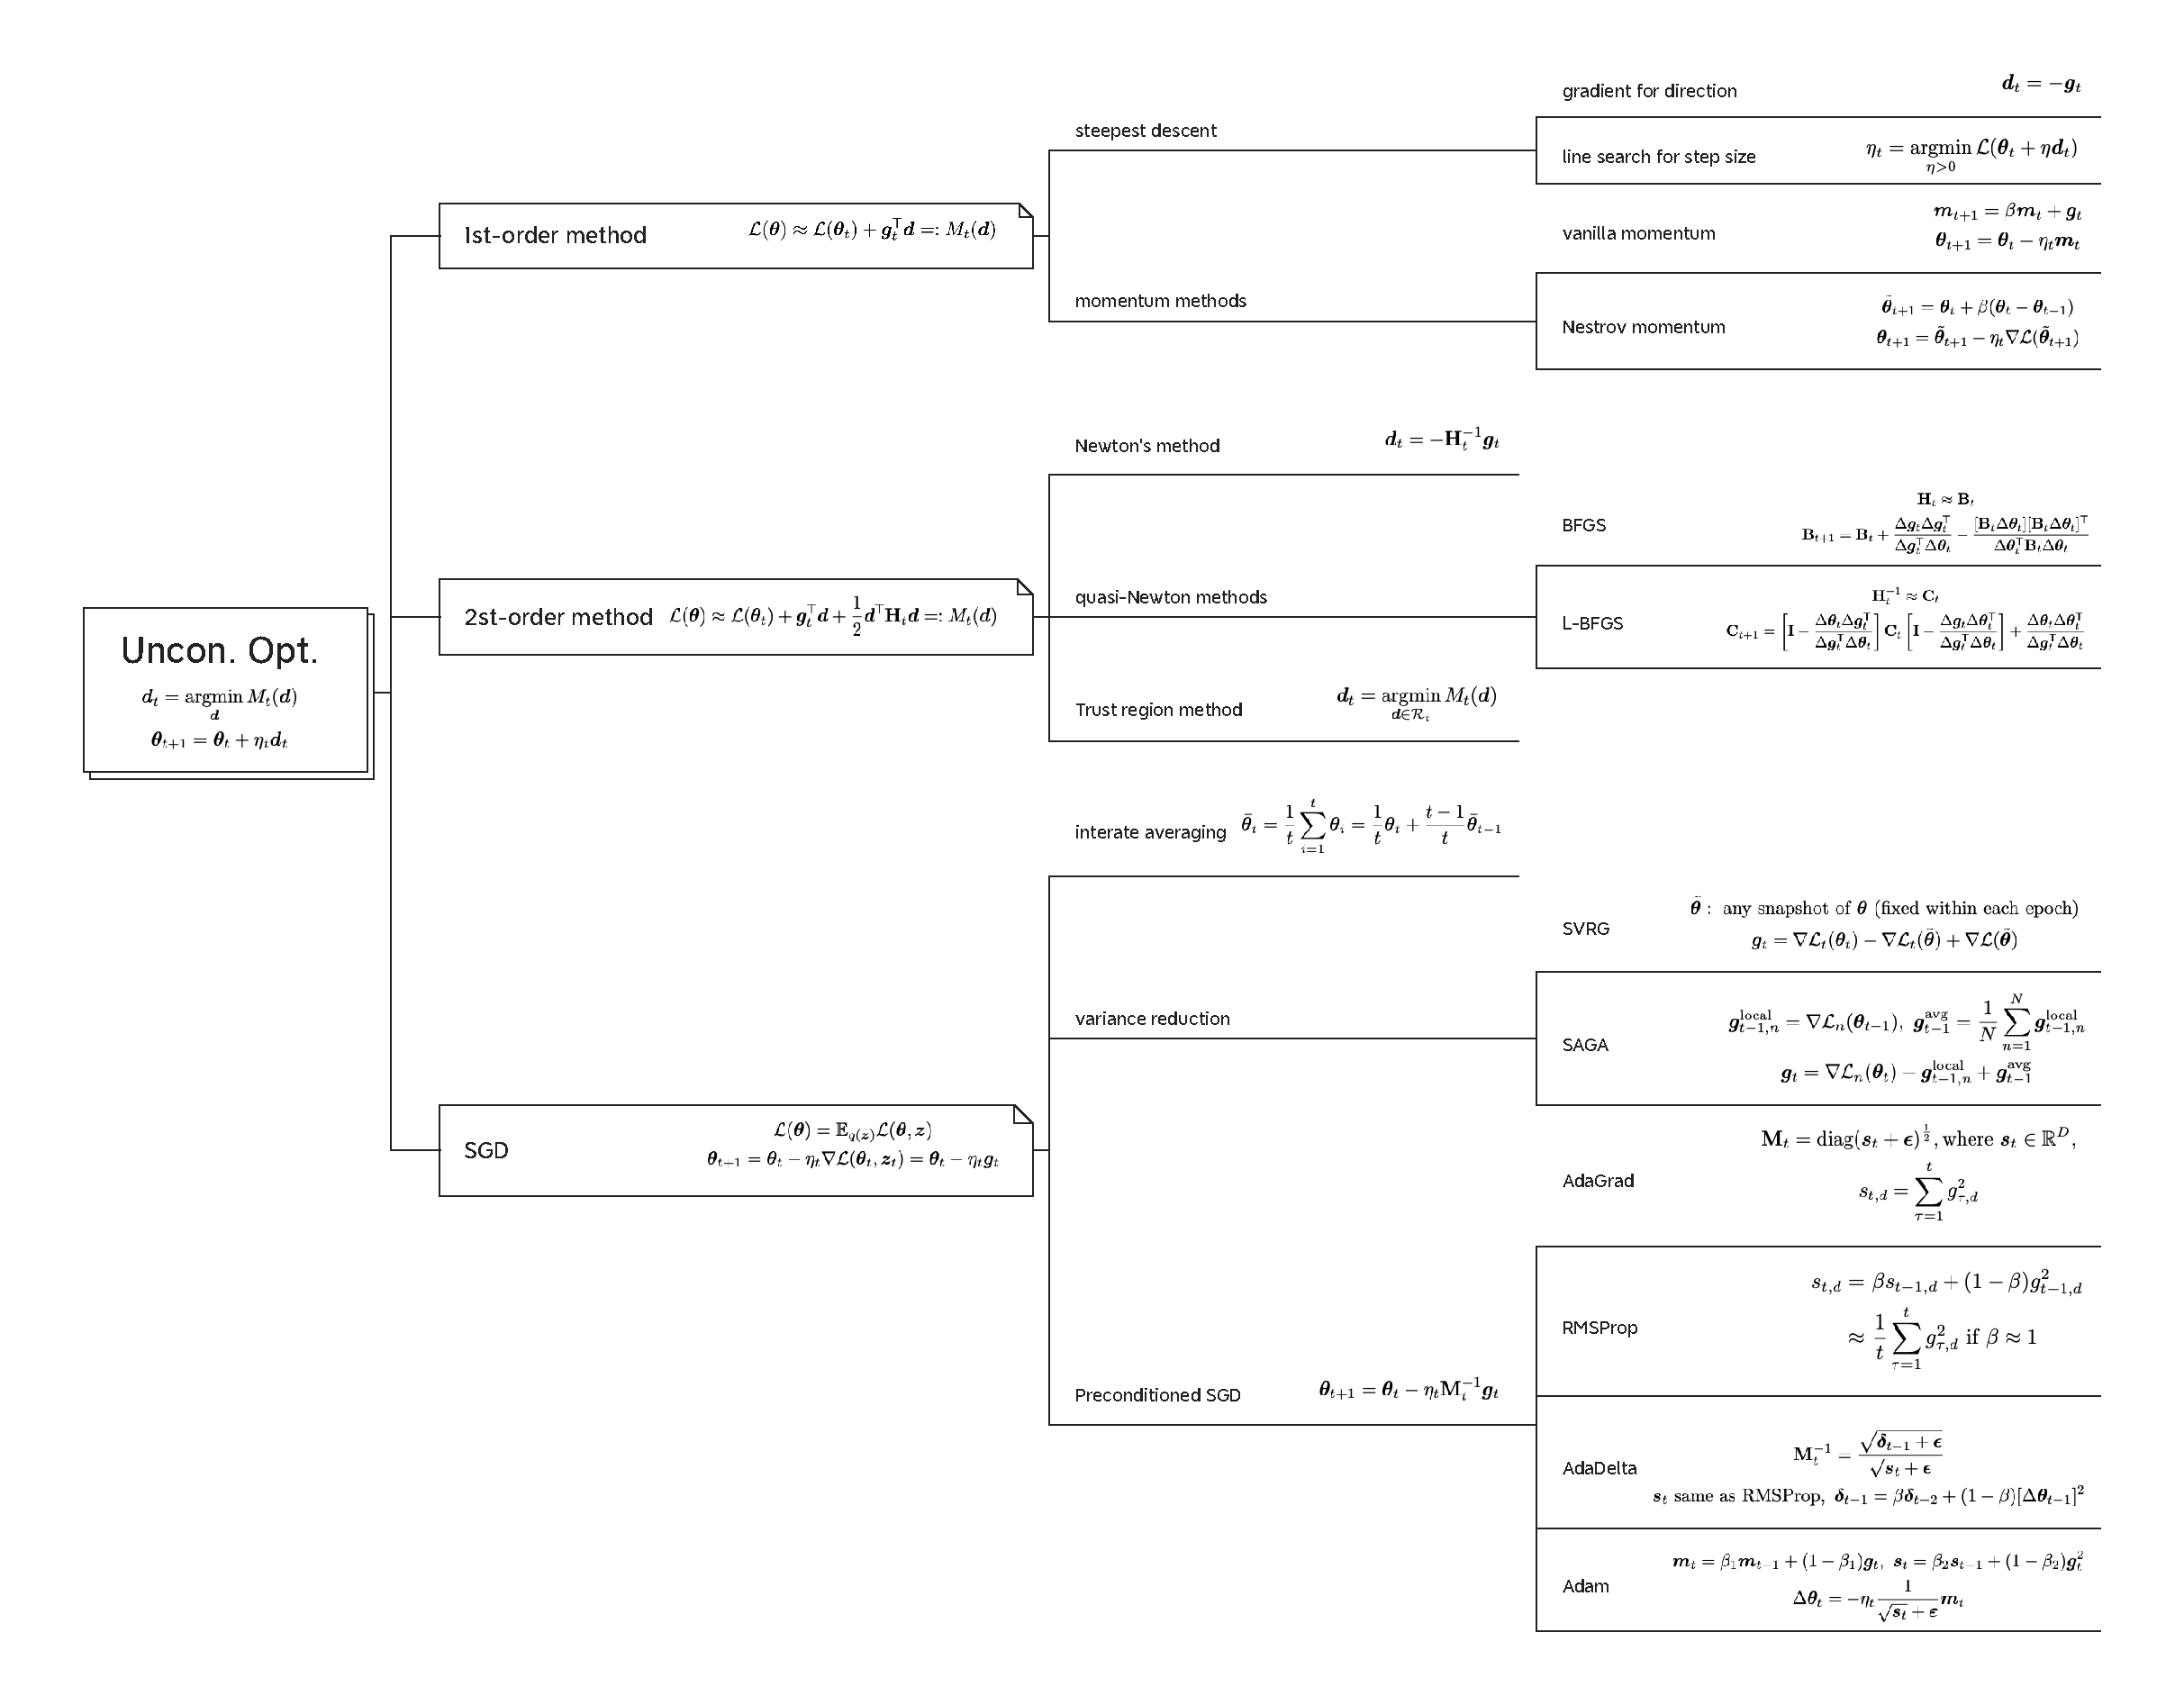
\includegraphics[width=\textwidth]{figs/unconopt.pdf}
    \caption{Solutions for unconstrained optimization updating strategies}
    {\footnotesize there are approximation methods for $M_t(\bm{d})$ and $\bm{d}_t$.
    \textbf{BFGS}: Broyden, Fletcher, Goldfarb and Shanno;
    \textbf{L-BFGS}: limited memory BFGS;
    \textbf{SGD}: Stochastic Gradient Descent;
    \textbf{SVRG}: Stochastic Variance Reduced Gradient;
    \textbf{SAGA}: Stochastic Averaged Gradient Accelerated;
    \textbf{AdaGrad}: ADAptive Gradient;
    \textbf{RMSProp}: Root Mean Squared resilient PROPagation;
    \textbf{Adam}: Adaptive moment estimation.
    }
    
    \label{fig:unconopt}
\end{figure}

% \textbf{Solutions for unconstrained optimization}: For updating strategy, 
% \begin{gather}
%     \bm{d}_t=\argmin_{\bm{d}}M_t(\bm{d})\\
%     \bm{\theta}_{t+1} = \bm{\theta}_t+\eta_t\bm{d}_t,
% \end{gather}
% there are approximation methods for $M_t(\bm{d})$ and $\bm{d}_t$
% \begin{itemize}
%     \item first-order methods 
%     \begin{gather}
%         \mathcal{L}(\bm{\theta})\approx\mathcal{L}(\bm{\theta}_t)+\bm{g}_t^\mathsf{T}\bm{d}=:M_t(\bm{d})
%     \end{gather}
%     \begin{itemize}
%         \item steepest descent
%         \begin{itemize}
%             \item gradient for direction 
%             \begin{gather}
%                 \bm{d}_t = -\bm{g}_t
%             \end{gather}
%             \item line search for step size 
%             \begin{gather}
%                 \eta_t = \argmin_{\eta>0}\mathcal{L}(\bm{\theta}_t+\eta\bm{d}_t)
%             \end{gather}
%         \end{itemize}
%         \item momentum methods
%         \begin{itemize}
%             \item vanilla momentum 
%             \begin{gather}
%             % \begin{cases}
%                 \bm{m}_{t+1} = \beta\bm{m}_t+\bm{g}_t \\
%                 \bm{\theta}_{t+1} = \bm{\theta}_t-\eta_t\bm{m}_t 
%             % \end{cases}
%             \end{gather}
%             \item Nestrov momentum 
%             \begin{gather}
%             % \begin{cases}
%                 \Tilde{\bm{\theta}}_{t+1} = \bm{\theta}_t+\beta(\bm{\theta}_t-\bm{\theta}_{t-1})\\
%                 \bm{\theta}_{t+1} = \Tilde{\bm{\theta}}_{t+1}-\eta_t\nabla\mathcal{L}(\Tilde{\bm{\theta}}_{t+1})
%             % \end{cases}
%             \end{gather}
%         \end{itemize}
%     \end{itemize}
%     \item second-order methods 
%     \begin{gather}
%         \mathcal{L}(\bm{\theta})\approx\mathcal{L}(\bm{\theta}_t)+\bm{g}_t^\mathsf{T}\bm{d}+\frac{1}{2}\bm{d}^\mathsf{T}\mathbf{H}_t\bm{d}=:M_t(\bm{d})
%     \end{gather}
%     \begin{itemize}
%         \item Newton's method 
%         \begin{gather}
%             \bm{d}_{t} = -\mathbf{H}_t^{-1}\bm{g}_t
%         \end{gather}
%         \item quasi-Newton's methods 
%         \begin{itemize}
%             \item BFGS
%             \begin{gather}
%             % \begin{cases}
%                 \mathbf{H}_t \approx \mathbf{B}_t\\
%                 \mathbf{B}_{t+1} = \mathbf{B}_t
%                    + \frac{\Delta\bm{g}_t\Delta\bm{g}_t^\mathsf{T}}{\Delta\bm{g}_t^\mathsf{T}\Delta\bm{\theta}_t}
%                    - \frac{[\mathbf{B}_t\Delta\bm{\theta}_t][\mathbf{B}_t\Delta\bm{\theta}_t]^\mathsf{T}}{\Delta\bm{\theta}_t^\mathsf{T}\mathbf{B}_t\Delta\bm{\theta}_t}
%             % \end{cases}
%             \end{gather}
%             \item L-BFGS
%             \begin{gather}
%             % \begin{cases}
%                 \mathbf{H}_t^{-1} \approx \mathbf{C}_t \\
%                 \mathbf{C}_{t+1} = 
%                     \left[
%                         \mathbf{I}-\frac{\Delta\bm{\theta}_t\Delta\bm{g}_t^\mathsf{T}}{\Delta\bm{g}_t^\mathsf{T}\Delta\bm{\theta}_t}
%                     \right]
%                     \mathbf{C}_t
%                     \left[
%                         \mathbf{I}-\frac{\Delta\bm{g}_t\Delta\bm{\theta}_t^\mathsf{T}}{\Delta\bm{g}_t^\mathsf{T}\Delta\bm{\theta}_t}
%                     \right]
%                     + \frac{\Delta\bm{\theta}_t\Delta\bm{\theta}_t^\mathsf{T}}{\Delta\bm{g}_t^\mathsf{T}\Delta\bm{\theta}_t}
%             % \end{cases}
%             \end{gather}
%         \end{itemize}
%         \item trust region method 
%         \begin{gather}
%             \bm{d}_t=\argmin_{\bm{d}\in\mathcal{R}_t}M_t(\bm{d})
%         \end{gather}
%     \end{itemize}
%     \item stochastic gradient descent (SGD)
%     \begin{gather}
%     % \begin{cases}
%         \mathcal{L}(\bm{\theta})=\mathbb{E}_{q(\bm{z})}\mathcal{L}(\bm{\theta},\bm{z})\\
%         \bm{\theta}_{t+1}=\bm{\theta}_t-\eta_t\nabla\mathcal{L}(\bm{\theta}_t,\bm{z}_t)=\bm{\theta}_t-\eta_t\bm{g}_t
%     % \end{cases}
%     \end{gather}
%     \begin{itemize}
%         \item iterate averaging 
%         \begin{gather}
%             \Bar{\bm{\theta}}_t=\frac{1}{t}\sum_{i=1}^t\bm{\theta}_i=\frac{1}{t}\bm{\theta}_t+\frac{t-1}{t}\Bar{\bm{\theta}}_{t-1}
%         \end{gather}
%         \item variance reduction
%         \begin{itemize}
%             \item stochastic variance reduced gradient (SVRG)
%             \begin{gather}
%             % \begin{cases}
%                 \Tilde{\bm{\theta}}:~\text{any snapshot of}~\bm{\theta}~\text{(fixed within each epoch)}\\
%                 \bm{g}_t=\nabla\mathcal{L}_t(\bm{\theta}_t)-\nabla\mathcal{L}_t(\Tilde{\bm{\theta}})+\nabla\mathcal{L}(\Tilde{\bm{\theta}})
%             % \end{cases}
%             \end{gather}
%             \item stochastic averaged gradient accelerated (SAGA)
%             \begin{gather}
%             \begin{cases}
%                 \bm{g}_{t-1,n}^\text{local}=\nabla\mathcal{L}_n(\bm{\theta}_{t-1})\\
%                 \bm{g}_{t-1}^\text{avg}=\frac{1}{N}\sum_{n=1}^N\bm{g}_{t-1,n}^\text{local}\\
%                 \bm{g}_t=\nabla\mathcal{L}_n(\bm{\theta}_t)-\bm{g}_{t-1,n}^\text{local}+\bm{g}_{t-1}^\text{avg}
%             \end{cases}
%             \end{gather}
%         \end{itemize}
%         \item preconditioned SGD ($\mathbf{M}_t$: preconditioner) 
%         \begin{gather}
%             \bm{\theta}_{t+1}=\bm{\theta}_t-\eta_t\mathbf{M}_t^{-1}\bm{g}_t
%         \end{gather}
%         \begin{itemize}
%             \item adaptive gradient (AdaGrad)
%             \begin{gather}
%                 \mathbf{M}_t=\mathrm{diag}(\bm{s}_t+\bm{\epsilon})^\frac{1}{2},\text{where}~\bm{s}_t\in\mathbb{R}^D,\\
%                 s_{t,d}=\sum_{\tau=1}^t g_{\tau,d}^2
%             \end{gather}
%             \item RMSProp
%             \begin{align}
%                 s_{t,d}
%                 =&~ \beta s_{t-1,d}+(1-\beta)g_{t-1,d}^2\\
%                 \approx&~ \frac{1}{t}\sum_{\tau=1}^t g_{\tau,d}^2~\text{if}~\beta\approx 1
%             \end{align}
%             \item AdaDelta
%             \begin{gather}
%                 \mathbf{M}_t^{-1}=\frac{\sqrt{\bm{\delta}_{t-1}+\bm{\epsilon}}}{\sqrt{\bm{s}_t+\bm{\epsilon}}}\\
%                 \bm{s}_t~\text{is the same as RMSProp}\\
%                 \bm{\delta}_{t-1}=\beta\bm{\delta}_{t-2}+(1-\beta)[\Delta \bm{\theta}_{t-1}]^2
%             \end{gather}
%             \item Adam
%             \begin{gather}
%                 \bm{m}_t=\beta_1\bm{m}_{t-1}+(1-\beta_1)\bm{g}_t\\
%                 \bm{s}_t=\beta_2\bm{s}_{t-1}+(1-\beta_2)\bm{g}_t^2\\
%                 \Delta\bm{\theta}_t=-\eta_t\frac{1}{\sqrt{\bm{s}_t}+\bm{\varepsilon}}\bm{m}_t
%             \end{gather}
%         \end{itemize}
%     \end{itemize}
% \end{itemize}


% \begin{note}
% \begin{enumerate}
%     \item condition number measures how ``skewed'' the space is, 
%     steepest descent converges much more quickly for the problem with the smaller condition number.
% \end{enumerate}
% \end{note}


\textbf{Bound optimization}: construct a surrogate target function $Q(\bm{\theta},\bm{\theta}_{t})$
\begin{gather}
    \bm{\theta}_{t+1}=\argmax_{\bm{\theta}}{Q(\bm{\theta},\bm{\theta}_{t})}\\
    \ell(\bm{\theta}_{t+1})\geq Q(\bm{\theta}_{t+1},\bm{\theta}_{t})\geq Q(\bm{\theta}_{t},\bm{\theta}_{t})=\ell(\bm{\theta}_{t})
\end{gather}

\textbf{EM algorithm}: $\bm{y}_n$ observed variables, $\bm{z}_n$ hidden variables, $\bm{\theta}$ parameters to estimate, 
and \textit{arbitrary} distributions $q_n(\bm{z}_n)$ for each sample
\begin{align}
    \ell(\bm{\theta})
    =& \sum_{n=1}^N\log{p(\bm{y}_n|\bm{\theta})} \\
    =& \sum_{n=1}^N\log\left[\sum_{\bm{z}_n}p(\bm{y}_n,\bm{z}_n|\bm{\theta})\right] \\
    =& \sum_{n=1}^N\log\left[\sum_{\bm{z}_n}q_n(\bm{z}_n)\frac{p(\bm{y}_n,\bm{z}_n|\bm{\theta})}{q_n(\bm{z}_n)}\right] \\
    =& \sum_{n=1}^N\log\left[\mathbb{E}_{q_n(\bm{z}_n)}\frac{p(\bm{y}_n,\bm{z}_n|\bm{\theta})}{q_n(\bm{z}_n)}\right] \\
    \geq& \sum_{n=1}^N\mathbb{E}_{q_n(\bm{z}_n)}\log\frac{p(\bm{y}_n,\bm{z}_n|\bm{\theta})}{q_n(\bm{z}_n)}~~\text{by Jensen} \\
    =& \underbrace{\sum_{n=1}^N\overbrace{
        \left[\mathbb{E}_{q_n(\bm{z}_n)}\log p(\bm{y}_n,\bm{z}_n|\bm{\theta})+\mathbb{H}(q_n(\bm{z}_n))\right]
    }^{\text{\L}(\bm{\theta},q_n)}}_{\text{\L}(\bm{\theta},q_{1:N})\text{:\textbf{evidence lower bound (ELBO)}}} \\
    =& \sum_{n=1}^N\mathbb{E}_{q_n(\bm{z}_n)}\log\frac{p(\bm{z}_n|\bm{y}_n,\bm{\theta})p(\bm{y}_n|\bm{\theta})}{q_n(\bm{z}_n)} \\
    =& \sum_{n=1}^N\left[
        \mathbb{E}_{q_n(\bm{z}_n)}\log\frac{p(\bm{z}_n|\bm{y}_n,\bm{\theta})}{q_n(\bm{z}_n)} 
        + \mathbb{E}_{q_n(\bm{z}_n)}\log p(\bm{y}_n|\bm{\theta})
    \right] \\
    =& \sum_{n=1}^N\left[
        -\infdiv{q_n(\bm{z}_n)}{p(\bm{z}_n|\bm{y}_n,\bm{\theta})} + \log p(\bm{y}_n|\bm{\theta})
    \right] \\
    =& \ell(\bm{\theta}) - \underbrace{\sum_{n=1}^N\infdiv{q_n(\bm{z}_n)}{p(\bm{z}_n|\bm{y}_n,\bm{\theta})}}_{\text{minimize the gap}}
\end{align}
\textbf{E step}: \unsure{
construct $Q(\bm{\theta},\bm{\theta}_{t})=\text{\L}(\bm{\theta},\{p(\bm{z}_n|\bm{y}_n,\bm{\theta}_{t})\}_{n=1}^{N})$
}
set 
\begin{gather}
    q_n(\bm{z}_n)=q_n^*:=p(\bm{z}_n|\bm{y}_n,\bm{\theta})
\end{gather} 
the \uline{posterior of each $\bm{z}_{n}$
given the observed data $\bm{y}_n$ and a \textit{initialized} $\bm{\theta}=\bm{\theta}^{(0)}$ or $\bm{\theta}=\bm{\theta}^{t}$ \textit{from previous step}}.
If the posterior cannot be computed exactly, then an approximate distribution is needed, yield a non-tight lower-bound.\\
\textbf{M step}: \unsure{
maximize the surrogate target $\text{\L}(\bm{\theta},\{p(\bm{z}_n|\bm{y}_n,\bm{\theta}_{t})\}_{n=1}^{N})$,
which is similar with MLE but the data of $\bm{z}_n$ is \textit{infinite} by providing its distribution.
And it can be viewed as decoupling the dependence to $\bm{y}_n\leftarrow\bm{\theta}$ and $\bm{z}_n\leftarrow\bm{\theta}_{t}$ only.
}
Denote $q^{(t)}_n(\bm{z}_n)=p(\bm{z}_n|\bm{y}_n,\bm{\theta}_{t})$, and we can get the \uline{expected complete data log likelihood} for current step
\begin{gather}
    \ell_{t}(\bm{\theta})=\sum_{n=1}^N\mathbb{E}_{q^{(t)}_n(\bm{z}_n)}\log p(\bm{y}_n,\bm{z}_n|\bm{\theta})\\
    \bm{\theta}_{t+1}=\argmax_{\bm{\theta}}\ell_{t}(\bm{\theta}).
\end{gather}
If the joint probability of $p(\bm{y}_n,\bm{z}_n|\bm{\theta})$ is in the exponential family,
i.e. 
\begin{gather}
    p(\bm{y}_n,\bm{z}_n|\bm{\theta})=h(\bm{y}_n,\bm{z}_n)\exp\{\mathcal{T}(\bm{y}_n,\bm{z}_n)^\mathsf{T}\bm{\theta}-A(\bm{\theta})\},
\end{gather}
then it can be simplified by the factorized terms in the index.




